\chapter{Kreisbewegung}
Bei einer Kreisbewegung verläuft die Bahnkurve kreisförmig,
d.h. die bewegte Masse hat eine zusammengesetzte Beschleunigung.
Diese setzt sich aus einem radialen und tangentialen Anteil 
zusammen. Da eine beschleunigte Masse eine Kraft ausübt, wird 
bei einer Kreisbewegung auch von Radial- bzw. Zentripetalkraft
(eine nach innen, zum Zentrum gerichtete Kraft) und der 
Tangentialkraft (eine tangential anliegende Kraft) gesprochen.

\section{Gleichförmige Kreisbewegung}
Bei einer gleichförmigen Kreisbewegung ist die Bahngeschwindigkeit
konstant und hat einen konstanten Abstand (Radius) zum Mittelpunkt.

\begin{figure}[h!]
	\centering
	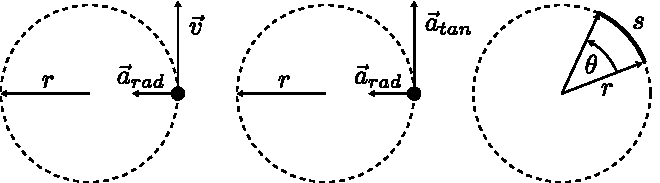
\includegraphics[scale=0.8]{kreisbewegung.pdf}
	\caption{Gleichförmige Kreisbewegung}
	\label{fig:kreisbewegung}
\end{figure}

\noindent
Die radial wirkende Kraft welche auch als Zentripetalkraft 
bezeichnet wird, kann auf verschiedene Weise berechnet werden.
\[ \boxed{\vec{F}_{rad} = \vec{F}_{ZP} 
	= m \cdot \vec{a}_{rad}
	= m \cdot \frac{\vec{v}^2}{r} 
	= m \cdot \omega^2 \cdot r 
	= m \cdot \frac{4 \cdot \pi^2 \cdot r}{T^2} } \]
Die Beziehungen zwischen den Bahngrössen lassen sich dabei 
grundsätzlich mit vier Gleichungen beschreiben:
\[ \boxed{ \begin{array}{l r l}
	\text{Bogenlänge $s$} & 
		s & = r \cdot \theta \\
	& & \\
	\text{Geschwindigkeit tangential $\vec{v}$} &
		\vec{v} & = r \cdot \omega
		= r \cdot \frac{d\omega}{dt} \\
	& & \\
	\text{Beschleunigung tangential $\vec{a}_{tan}$} &
		\vec{a}_{tan} & = r \cdot \alpha 
		= r \cdot \frac{d^2\theta}{dt} \\
	& & \\
	\text{Beschleunigung radial $\vec{a}_{rad}$} &
		\vec{a}_{rad} & = \frac{v^2}{r} = \omega^2 \cdot r
\end{array} }\]

\noindent
Wichtig ist der Zusammen zwischen den verschiedenen Beschleunigungen
eines Rotierenden Körpers zu beachten.
\[ \boxed{\begin{array}{r l}
	\vec{a}_{rad} & = \frac{\vec{v}^2}{r} 
		= \omega^2 \cdot r 
		= \dot{\omega}^2 \cdot r \\
	& \\
	\vec{a}_{tan} & = \alpha \cdot r
		= \ddot{\omega} \cdot r \\
	& \\
	\vec{a}_{res} & = \sqrt{\vec{a}_{rad}^2 + \vec{a}_{tan}^2} 
\end{array} }\]

\section{Winkelbetrachtung}\label{sec:winkelbetrachtung}
Bei Kreisbewegungen ist es von Vorteil, wenn die Bewegung nicht als
Weg pro Zeit ($\frac{m}{s}$) sondern als Winkel pro Zeit 
($\frac{rad}{s}$) betrachtet wird. Eine Kreisbewegung kann somit 
unabhängig vom Radius beschrieben werden. In diesem Fall spricht
man dann von der Winkelgeschwindigkeit $\omega$ und 
Winkelbeschleunigung $\alpha$. Mit dieser Betrachtungsweise kann
eine Kreisbewegung analog zur Translation beschrieben werden, denn
auch hier gilt der Zusammenhang von Weg, Geschwindigkeit und 
Beschleunigung wie in der Translation.

\[ \boxed{ \begin{array}{l l}
	\text{Rotation} \qquad &
		\theta
		\xrightarrow{\frac{d}{dt}} \omega 
		\xrightarrow{\frac{d}{dt}} \alpha \\
	& \\
	\text{Translation} \qquad &
		s
		\xrightarrow{\frac{d}{dt}} \vec{v} 
		\xrightarrow{\frac{d}{dt}} \vec{a}
\end{array} }\]

\noindent
Die einzelnen Grössen $\omega$ und $\alpha$ können mit den folgenden 
Formeln beschrieben werden.
\[ \boxed{\begin{array}{l r l}
	\text{Winkelgeschwindigkeit} &
		\omega & = \omega_0 + \alpha \cdot t 
			= \frac{d\theta}{dt} 
			= \dot{\theta} \\
	& & \\
	\text{Winkelbeschleunigung} &
		\alpha & = \frac{d^2\theta}{dt^2} = \ddot{\theta}
\end{array} }\]

\section{Trägheitsmoment}
Das Trägheitsmoment beschreibt die Massenverteilung eines Körpers
bezogen auf eine Drehachse. Dieses muss bei jeder Form von Rotation
berücksichtigt werden und ist grundsätzlich unabhängig von der 
Bewegung, nicht aber von der Drehachse.

Das Trägheitsmoment wird beschrieben durch die Summe der 
Produkte aus den Massepunkten und deren Abstand im Quadrat zur 
Drehachse des Körpers.
\[ \boxed{
	I = m_1 \cdot r_1^2
		+ m_2 \cdot r_2^2 
		+ \dots 
		+ m_n \cdot r_n^2
		= \sum m_i \cdot r_i^2
		= \int r^2 \cdot dm
} \]

\noindent
Trägheitsmomente verschiedener Körper können zu einem Trägheitsmoment
summiert werden, wenn diese auf der gleichen Drehachse rotieren.
\[ \boxed{
	I_{Total} = I_1 + I_2 + \dots + I_n
} \]

\section{Rotationsenergie}
Die Rotationsenergie ist im Grunde genommen die kinetische Enerige
eines starren Körpers der um eine feste Achse rotiert.
\[ \boxed{\begin{array}{r l}
	E_{kin} & = \frac{1}{2} \cdot m \cdot \vec{v}^2 \\
	& \\
	\Rightarrow E_{rot} & = \frac{1}{2} \cdot m_1 \cdot \vec{v}_1^2
			+ \frac{1}{2} \cdot m_2 \cdot \vec{v}_2^2
			+ \dots 
			+ \frac{1}{2} \cdot m_n \cdot \vec{v}_n^2 \\
	& \\
		& = \frac{1}{2} \cdot \left(m_1 \cdot r_1^2
			+ m_2 \cdot r_2^2 
			+ \dots
			+ m_n \cdot r_n^2\right) \cdot \omega^2 \\
	& \\
		& = \frac{1}{2} \cdot I \cdot \omega^2 
\end{array} } \]

\newpage
\section{Rotation vs. Translation}
Wie im Kapitel \ref{sec:winkelbetrachtung} beschrieben, kann die 
Rotation analog zur Translation betrachtet werden.

\[ \boxed{\begin{array}{l l}
\textbf{Rotation} & \textbf{Translation} \\
& \\
\text{Winkelbeschleunigung $\left[\frac{rad}{s^2}\right]$}
	& \text{Beschleunigung $\left[\frac{m}{s^2}\right]$} \\
		\qquad \alpha = \frac{d^2\theta}{dt^2} = \ddot{\theta}
			& \qquad \vec{a} = \frac{d^2s}{dt^2} \\
& \\
\text{Winkelgeschwindigkeit $\left[\frac{rad}{s}\right]$} 
	& \text{Geschwindigkeit $\left[\frac{m}{s}\right]$} \\
		\qquad \omega = \frac{d\theta}{dt} = \dot{\theta} 
			& \qquad \vec{v} = \frac{ds}{dt} \\
& \\
\text{Winkel $\left[rad\right]$} 
	& \text{Weg $\left[ m \right]$} \\
		\qquad \theta = \omega_0 \cdot t + \frac{1}{2} \cdot \alpha \cdot t^2
			& \qquad s = \vec{v}_0 \cdot t + \frac{1}{2} \cdot \vec{a} \cdot t^2 \\
		& \\
		\qquad \theta = \frac{1}{2} \cdot (\omega + \omega_0) \cdot t
			& \qquad s = \frac{1}{2} \cdot (\vec{v} + \vec{v}_0) \cdot t \\
& \\
\text{Trägheitsmoment $\left[kg \cdot m^2\right]$} 
	& \text{Masse $\left[kg\right]$} \\
		\qquad I = \sum r_i^2 \cdot m_i = \int r^2 \cdot dm
			& \qquad m \\
& \\
\text{Drehmoment $\left[N \cdot m\right]$}
	& \text{Kraft $\left[N\right]$} \\
		\qquad M = I \cdot \alpha
			& \qquad \vec{F} = m \cdot \vec{a} \\
& \\
\text{Drehimpuls $\left[\frac{kg \cdot m^2}{s}\right]$} 
	& \text{Impuls $\left[N \cdot s\right]$} \\
		\qquad L = I \cdot \omega
			& \qquad \vec{p} = m \cdot \vec{a} \\
& \\
\text{Rotationsenergie $\left[J\right]$} 
	& \text{Kinetische Energie $\left[J\right]$} \\
		\qquad E_{Rot} = \frac{1}{2} \cdot I \cdot \omega^2
			& \qquad E_{Kin} = \frac{1}{2} \cdot m \cdot \vec{v}^2 \\
& \\
\text{Leistung $\left[W\right]$}
	& \text{Leistung $\left[W\right]$} \\
		\qquad P = \frac{dE}{dt} = M \cdot \omega 
			& \qquad P = \vec{F} \cdot \vec{v}
\end{array} } \]


